\documentclass[12pt, a4paper]{article}

% ─── Packages ─────────────────────────────────────────────
\usepackage[utf8]{inputenc}
\usepackage[T1]{fontenc}
\usepackage[english]{babel}
\usepackage{lmodern}
\usepackage[left=2.5cm, right=2.5cm, top=2.5cm, bottom=2.5cm]{geometry}
\usepackage{setspace}
\usepackage{parskip}
\usepackage{enumitem}
\usepackage{booktabs}
\usepackage{tabularx}
\usepackage{array}
\usepackage{hyperref}
\usepackage{amsmath}
\usepackage{csquotes}
\usepackage{xcolor}
\usepackage{titlesec}
\usepackage{tikz}
\usepackage{float}

\usetikzlibrary{arrows.meta, positioning, shapes.geometric, fit, backgrounds, calc}

\hypersetup{
    colorlinks=true,
    linkcolor=black,
    citecolor=blue!60!black,
    urlcolor=blue!60!black,
}

\onehalfspacing

% ─── Colors ───────────────────────────────────────────────
\definecolor{inputcolor}{HTML}{E3F2FD}
\definecolor{corecolor}{HTML}{FFF3E0}
\definecolor{outputcolor}{HTML}{E8F5E9}
\definecolor{compbg}{HTML}{F5F5F5}
\definecolor{compborder}{HTML}{9E9E9E}
\definecolor{accentblue}{HTML}{1565C0}
\definecolor{accentorange}{HTML}{E65100}
\definecolor{accentgreen}{HTML}{2E7D32}

% ─── Title ────────────────────────────────────────────────
\title{%
    \vspace{-1cm}
    \textbf{Master's Thesis --- Outline}\\[0.8em]
    \Large Cost-Efficient Modeling of Multi-Stakeholder\\
    Problems via LLM-Based Agent Simulation:\\[0.3em]
    Design, Implementation, and Evaluation\\
    of a Cost-Optimized Framework\\[1em]
    \normalsize\textit{Master's Thesis in Computer Science}
}

\author{Janik H\"ausser}
\date{June 2026}

% ──────────────────────────────────────────────────────────
\begin{document}

\maketitle
\thispagestyle{empty}

\newpage
\setcounter{page}{1}

% ══════════════════════════════════════════════════════════
\section{Objectives}
% ══════════════════════════════════════════════════════════

The goal of this thesis is the design, implementation, and evaluation of an end-to-end framework for LLM-based multi-agent simulations. From declarative scenario definition through agent modeling to automated analysis. The framework will be evaluated using a concrete use case (peatland rewetting) and shall exhibit the following core properties:

\begin{enumerate}
    \item \textbf{Declarative scenario and persona definition}: Stakeholders, personas (including background, goals, constraints), interaction rules, and incentive mechanisms are specified via structured configuration (YAML/JSON Schema) without code changes.

    \item \textbf{Cost optimization}: Systematic reduction of API costs through:
    \begin{itemize}
        \item prompt compression and token budgeting,
        \item intelligent model routing (cheaper models for simpler sub-tasks),
        \item prompt caching and response memoization,
        \item structured output modes (reducing parsing errors and retries).
    \end{itemize}

    \item \textbf{Performance and scalability}: Efficient parallelization, batching, and rate-limit management for large cohorts.

    \item \textbf{Scientific rigor}: Reproducibility through seed control, configuration snapshotting, complete audit trails, and a standardized analysis pipeline.

    \item \textbf{Multi-provider support}: Abstraction of the LLM interface to support multiple providers (OpenAI, Anthropic, Mistral, local models via Ollama).
\end{enumerate}

% ══════════════════════════════════════════════════════════
\section{Research Questions}
% ══════════════════════════════════════════════════════════

\subsection*{Main Question}

\begin{quote}
    \textit{How can a generic, cost-efficient framework for LLM-based multi-agent simulations of stakeholder negotiations be designed, implemented, and evaluated?}
\end{quote}

\subsection*{Sub-Questions}

\begin{description}[style=nextline, leftmargin=1.5cm]
    \item[RQ1 (Cost Optimization: Core)] Which specific optimization strategies (structured output, prompt compression, model routing, response caching, local models) reduce per-simulation costs, and what is their individual and cumulative impact on cost and decision quality?

    \item[RQ2 (Cost-Quality Tradeoff)] What is the relationship between cost reduction and result quality across optimization strategies? Is there a cost--quality sweet spot where significant savings can be achieved with minimal quality degradation?

    \item[RQ3 (Architecture)] How must the framework architecture be designed so that different stakeholder scenarios (negotiation, iterative game, multi-stakeholder conflict) can be modeled through configuration changes alone, with optimization strategies switchable via configuration?

    \item[RQ4 (Validity \& Reproducibility)] As a necessary precondition for meaningful cost comparisons: Do LLM-based agents produce sufficiently plausible and reproducible decisions, and how sensitive are results to model choice, temperature, and prompt variations?
\end{description}

% ══════════════════════════════════════════════════════════
\section{Framework Architecture Overview}
\label{sec:architecture}
% ══════════════════════════════════════════════════════════

The framework follows a \textbf{three-layer architecture}: an input layer for declarative configuration, a core engine for orchestration and LLM interaction, and an output layer for structured, reproducible results.

\begin{figure}[H]
\centering
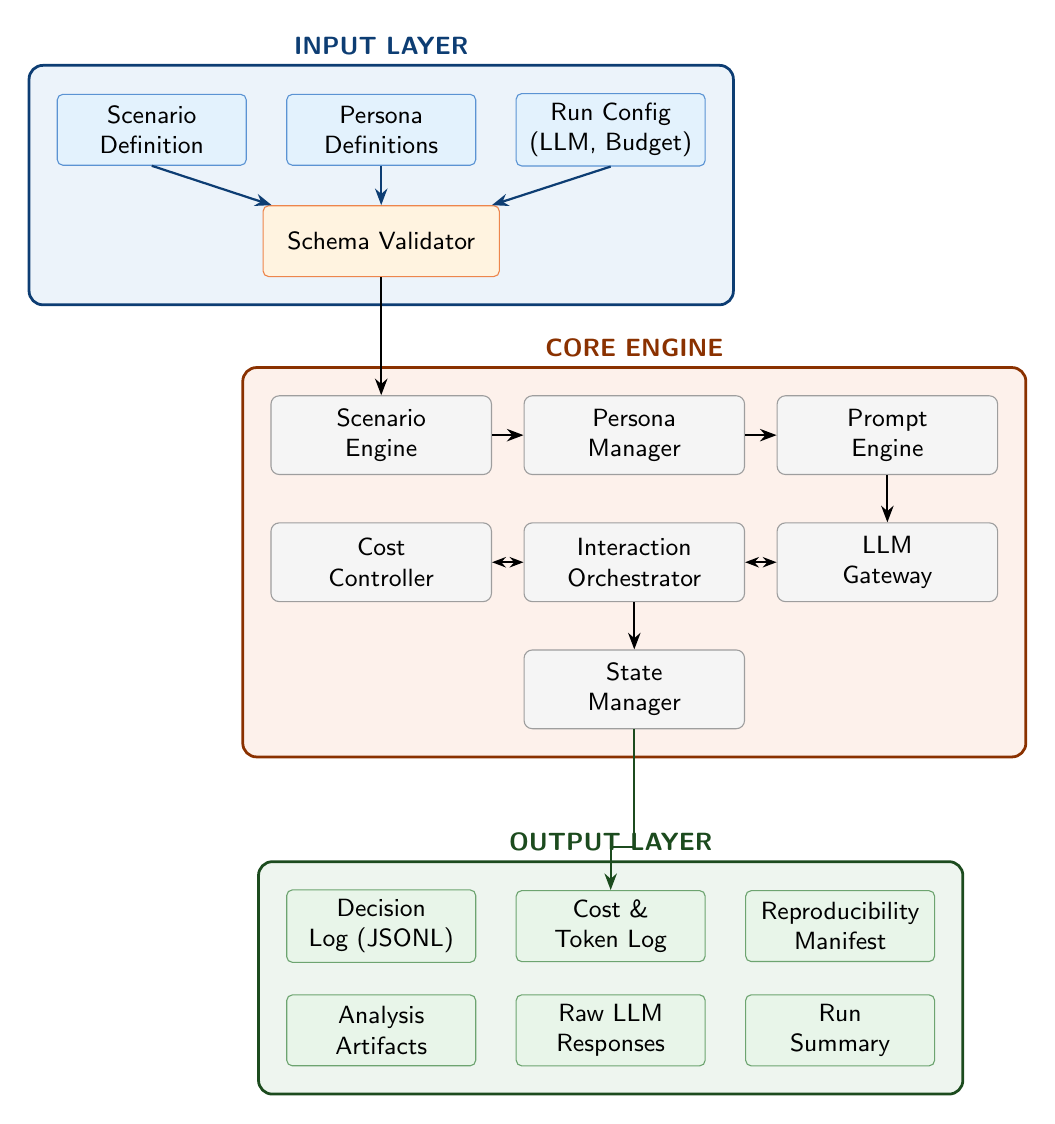
\begin{tikzpicture}[node distance=0.6cm and 0.8cm,
    component/.style={rectangle, draw=compborder, fill=compbg, rounded corners=3pt,
                      minimum height=1cm, minimum width=2.8cm, align=center, font=\small\sffamily},
    layer box/.style={rectangle, draw=#1!60!black, fill=#1!8,
                      rounded corners=5pt, inner sep=10pt, line width=1pt},
    layer label/.style={font=\small\sffamily\bfseries, text=#1!60!black},
    data flow/.style={-{Stealth[length=6pt]}, thick, color=#1!60!black},
    data flow/.default={black},
    bidirectional/.style={{Stealth[length=5pt]}-{Stealth[length=5pt]}, thick, color=#1!60!black},
    bidirectional/.default={black},
    input file/.style={rectangle, draw=accentblue!70, fill=inputcolor,
                       rounded corners=2pt, minimum height=0.9cm,
                       minimum width=2.4cm, align=center, font=\small\sffamily},
    output file/.style={rectangle, draw=accentgreen!70, fill=outputcolor,
                        rounded corners=2pt, minimum height=0.9cm,
                        minimum width=2.4cm, align=center, font=\small\sffamily},
    process/.style={rectangle, draw=accentorange!70, fill=corecolor,
                    rounded corners=2pt, minimum height=0.9cm,
                    minimum width=2.4cm, align=center, font=\small\sffamily},
]

    % ── Input Layer ──
    \node[input file] (scenario) {Scenario\\Definition};
    \node[input file, right=0.5cm of scenario] (personas) {Persona\\Definitions};
    \node[input file, right=0.5cm of personas] (runconfig) {Run Config\\(LLM, Budget)};

    \node[process, below=0.5cm of personas, minimum width=3cm] (validator) {Schema Validator};

    \begin{scope}[on background layer]
        \node[layer box=accentblue, fit=(scenario)(personas)(runconfig)(validator),
              label={[layer label=accentblue]above:INPUT LAYER}] (inputlayer) {};
    \end{scope}

    \draw[data flow=accentblue] (scenario.south) -- (validator);
    \draw[data flow=accentblue] (personas.south) -- (validator);
    \draw[data flow=accentblue] (runconfig.south) -- (validator);

    % ── Core Engine ──
    \node[component, below=1.5cm of validator] (sceneng) {Scenario\\Engine};
    \node[component, right=0.4cm of sceneng] (persmgr) {Persona\\Manager};
    \node[component, right=0.4cm of persmgr] (prompteng) {Prompt\\Engine};

    \node[component, below=0.6cm of sceneng] (costctrl) {Cost\\Controller};
    \node[component, right=0.4cm of costctrl] (orchestrator) {Interaction\\Orchestrator};
    \node[component, right=0.4cm of orchestrator] (llmgw) {LLM\\Gateway};

    \node[component, below=0.6cm of orchestrator] (statemgr) {State\\Manager};

    \begin{scope}[on background layer]
        \node[layer box=accentorange,
              fit=(sceneng)(persmgr)(prompteng)(costctrl)(orchestrator)(llmgw)(statemgr),
              label={[layer label=accentorange]above:CORE ENGINE}] (corelayer) {};
    \end{scope}

    \draw[data flow] (validator) -- (sceneng);
    \draw[data flow] (sceneng) -- (persmgr);
    \draw[data flow] (persmgr) -- (prompteng);
    \draw[data flow] (prompteng) -- (llmgw);
    \draw[bidirectional] (costctrl) -- (orchestrator);
    \draw[bidirectional] (orchestrator) -- (llmgw);
    \draw[data flow] (orchestrator) -- (statemgr);

    % ── Output Layer ──
    \node[output file] (declog) at ([yshift=-2.5cm]statemgr.south -| costctrl.center) {Decision\\Log (JSONL)};
    \node[output file, right=0.5cm of declog] (costlog) {Cost \&\\Token Log};
    \node[output file, right=0.5cm of costlog] (manifest) {Reproducibility\\Manifest};

    \node[output file, below=0.4cm of declog] (analysis) {Analysis\\Artifacts};
    \node[output file, right=0.5cm of analysis] (rawresp) {Raw LLM\\Responses};
    \node[output file, right=0.5cm of rawresp] (summary) {Run\\Summary};

    \begin{scope}[on background layer]
        \node[layer box=accentgreen,
              fit=(declog)(costlog)(manifest)(analysis)(rawresp)(summary),
              label={[layer label=accentgreen]above:OUTPUT LAYER}] (outputlayer) {};
    \end{scope}

    \draw[data flow=accentgreen] (statemgr.south) -- ++(0,-1.5) -| (costlog.north);

\end{tikzpicture}
\caption{Architecture of the simulation framework.}
\label{fig:arch}
\end{figure}

\subsection*{Input Layer}

Three YAML configuration files define a simulation, each validated against a JSON Schema:
\begin{itemize}
    \item \textbf{Scenario definition}: stakeholder roles, interaction rules (topology, round logic, visibility), incentive mechanisms, target metrics, and global constraints.
    \item \textbf{Persona definitions}: per-agent background, goals, risk profile, weighted decision factors, and personality traits. Separated from the scenario to enable reuse and combinatorial studies.
    \item \textbf{Run configuration}: LLM provider selection, model routing rules, retry logic, cost budgets, caching strategy, parallelism, and seed.
\end{itemize}

\subsection*{Core Engine}

The core engine consists of six components:
\begin{enumerate}
    \item \textbf{Scenario Engine}: parses and validates the input files, resolves persona-to-role assignments (seeded for reproducibility).
    \item \textbf{Persona Manager}: instantiates agents by rendering system prompts from persona definitions and scenario context.
    \item \textbf{Interaction Orchestrator}: executes the simulation loop for each round: build per-agent context, render prompts, issue LLM calls (parallel or sequential), parse and validate responses, update immutable state, log results, and check termination conditions.
    \item \textbf{LLM Gateway}: unified provider interface built on \texttt{litellm} or \texttt{langchain}, providing transparent access to different remote models (OpenAI, Mistral, etc.), and local models (via Ollama). Includes cost-saving features such as cache lookup, model routing, and budget enforcement before each call.
    \item \textbf{Cost Controller}: tracks token usage and cost per API call, enforces hard budget limits, and triggers warnings or aborts at configurable thresholds.
    \item \textbf{State Manager}: maintains immutable per-round state snapshots, enabling full traceability and safe parallelization.
\end{enumerate}

\subsection*{Output Layer}

Structured outputs include:
\begin{itemize}
    \item \textbf{Decision logs}: one entry per agent per round, including the decision, reasoning, token usage, cost, latency, and model used.
    \item \textbf{Cost logs}: granular per-call cost tracking with cache hit status.
    \item \textbf{Reproducibility manifest}: config hash, seed, framework version and exact LLM model versions used.
    \item \textbf{Run summary}: aggregated results across repetitions (e.g., acceptance rates per persona, cost per simulation).
    \item \textbf{Config snapshot}: exact copy of all input files for full reproducibility.
\end{itemize}

\subsection*{Key Cost Optimization Strategies}

\begin{table}[H]
    \centering
    \small
    \begin{tabularx}{\textwidth}{lX}
        \toprule
        \textbf{Strategy} & \textbf{Mechanism}\\
        \midrule
        Structured output    & JSON mode / tool-use to eliminate parse retries \\
        Prompt compression   & Summarize history in late rounds \\
        Model routing        & Strong model for decisions, cheap for summaries \\
        Response caching     & SHA-256 hash over prompt $\to$ cache lookup \\
        Batch API            & OpenAI Batch API (50\% discount, 24h SLA)                    \\
        Local models         & Ollama for development and testing                            \\
        \bottomrule
    \end{tabularx}
    \caption{Cost optimization strategies (exact measurements are part of the evaluation).}
    \label{tab:cost}
\end{table}

% ══════════════════════════════════════════════════════════
\section{Preliminary Timeline}
% ══════════════════════════════════════════════════════════

\begin{table}[h!]
    \centering
    \begin{tabularx}{\textwidth}{llX}
        \toprule
        \textbf{Phase} & \textbf{Period} & \textbf{Tasks} \\
        \midrule
        1.\ Analysis
            & Month 1--2
            & Literature review, requirements analysis, domain analysis of peatland scenario, benchmark definition, analysis of prototype \\
        2.\ Design
            & Month 2--3
            & Architecture design, schema design, technology selection \\
        3.\ Implementation
            & Month 3--5
            & Core framework, persona modeling, LLM integration, cost optimization strategies (each as config-switchable feature), tests \\
        4.\ Evaluation
            & Month 4--5
            & Waterfall cost experiment, model comparison, peatland simulation, reproducibility tests \\
        5.\ Writing
            & Month 2--6
            & Continuous writing from Month~2 (design chapter first); main writing phase Month~5--6 \\
        \bottomrule
    \end{tabularx}
    \caption{Preliminary timeline (assumption: 6-month thesis period).}
    \label{tab:timeline}
\end{table}

\end{document}
